\section{Question 3}

\begin{question}
    Performing a 10-fold Stratified Cross-Validation, what is the impact the minimal gain and maximal
    depth parameters on the average accuracy achieved by Decision Tree? Report at least 5 screenshots
    showing the confusion matrices achieved using different parameter settings (consider at least all
    the configurations used to answer Question 2). Keep the default configuration for all the other
    parameters.
\end{question}

\begin{answer}
    \\
    Figure 6 shows how the impact of having a fixed \textbf{maximal depth} to 1000, and decreasing
    the value of the \textbf{minimal gain}. It can be seen that the lower its value, the recall for the
    recurrence-events class increases, and the precision decreases. While for the no-recurrence-events,
    the recall decreases and the precision increases. Note also that values stabilizes after 0.001,
    which do not change for the values with a \textbf{minimal gain} of 1x10-5.
    \\
    \\

    \begin{figure}
        \centering
        \subfigure[]{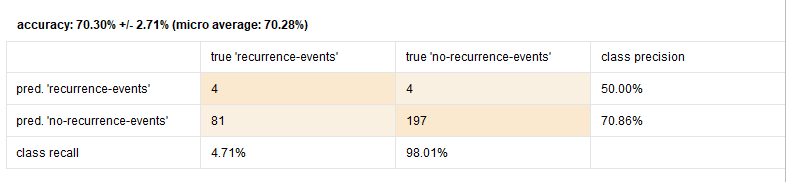
\includegraphics[width=0.48\textwidth]{Screenshot_15.png}}
        \subfigure[]{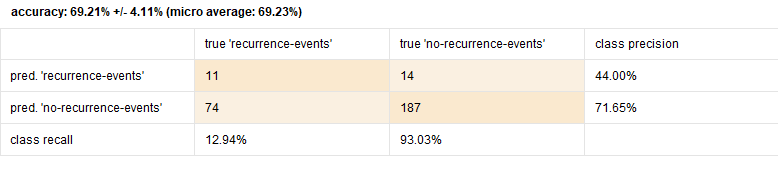
\includegraphics[width=0.48\textwidth]{Screenshot_16.png}}
        \subfigure[]{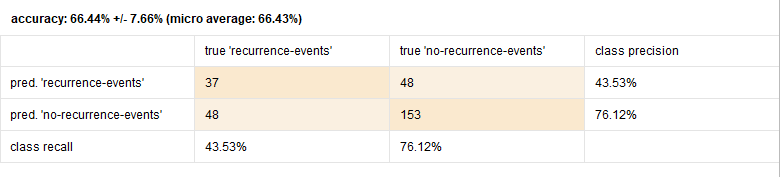
\includegraphics[width=0.48\textwidth]{Screenshot_17.png}}
        \subfigure[]{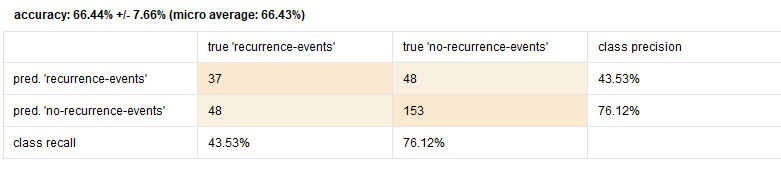
\includegraphics[width=0.48\textwidth]{Screenshot_18.png}}
        \caption{Impact of the \textbf{minimal gain} with values (maximal depth fixed to 1000)
            \\
            (a) 0.065 (b) 0.06 (c) 0.001 (d) 1x1e-5}
    \end{figure}
    Figure 6, shows how the \textbf{maximal depth} improves the model. More the max depth, the recall and
    precision balance improves.
    \begin{figure}
        \centering
        \subfigure[]{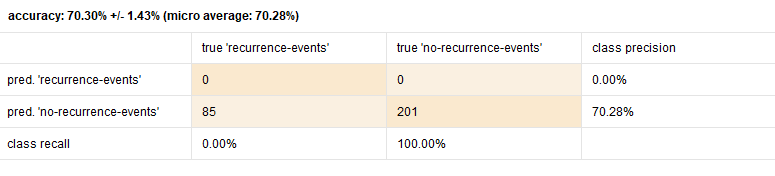
\includegraphics[width=0.48\textwidth]{Screenshot_19.png}}
        \subfigure[]{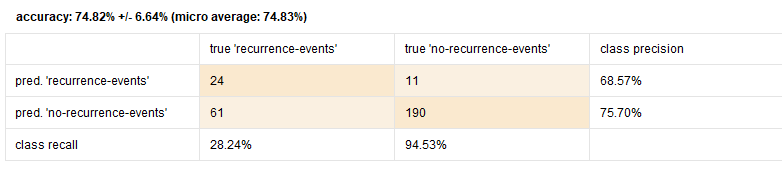
\includegraphics[width=0.48\textwidth]{Screenshot_20.png}}
        \subfigure[]{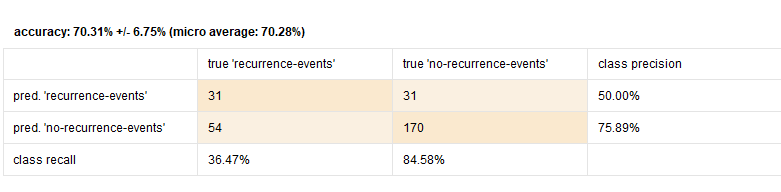
\includegraphics[width=0.48\textwidth]{Screenshot_21.png}}
        \subfigure[]{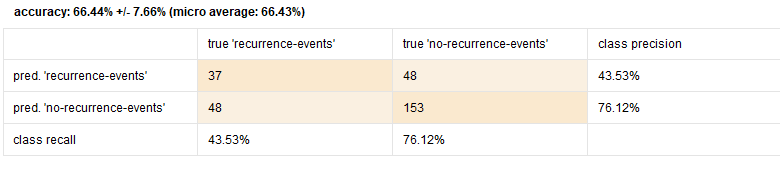
\includegraphics[width=0.48\textwidth]{Screenshot_22.png}}
        \caption{Impact of the \textbf{maximal depth} with values (minimal gain fixed to 0.001)
            \\
            (a) 1 (b) 3 (c) 4 (d) 1000}
    \end{figure}
    Figure 7 reforce the fact that the depth of the project does not mean a more balanced model. While a
    minimal gain actually does improve the balance of the model.
    \begin{figure}
        \centering
        \subfigure[]{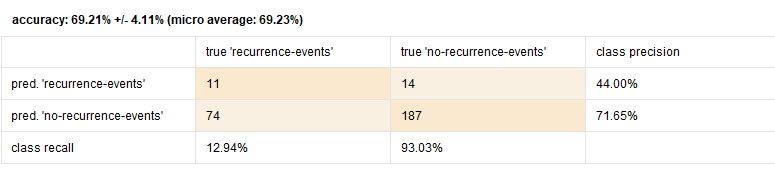
\includegraphics[width=0.48\textwidth]{Screenshot_23.png}}
        \subfigure[]{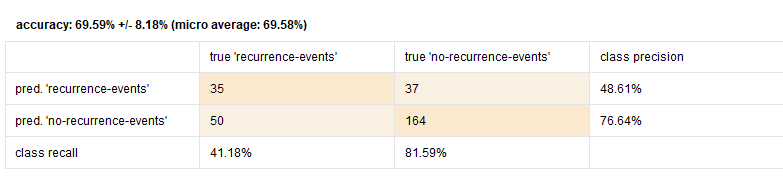
\includegraphics[width=0.48\textwidth]{Screenshot_24.png}}
        \caption{Impact of the \textbf{maximal depth} \textbf{minimal gain}
        \\
        (a) minimal gain: 0.06 maximal depth: 1000 (b) minimal gain: 1x10-5 maximal depth: 5}
    \end{figure}
\end{answer}
\pagebreak